\documentclass{scrreprt}
\usepackage[utf8]{inputenc}
\usepackage[T1]{fontenc}
\usepackage{lmodern}
\usepackage[francais]{babel, varioref}
\usepackage{graphicx}
\usepackage{listings}
%\usepackage[pdfborder={0 0 0},
 %           pdfcreator={},
   %         pdfsubject={Projet Correcteur orthographique},
  %          pdftitle={Projet Correcteur orthographique}]{hyperref}
\usepackage{xspace}
\usepackage{amssymb}
\usepackage{calc}
\usepackage{listingsutf8}
\usepackage{color}
\usepackage{xcolor}

%%%%%%%%%%%%%%%%%%%%%
\usepackage{url}
\usepackage[top=2.1cm,bottom=2.2cm,left=2cm,right=2cm]{geometry}
\usepackage[final]{pdfpages}
%%%%%%%%%%%%%%%%%%%%%%%%%%%

%%%%%%%%%%% Pour sommaire cliquable %%%%%%%%%%
\usepackage{hyperref} % Créer des liens et des signets
\hypersetup{
colorlinks=true, %colorise les liens
breaklinks=true, %permet le retour à la ligne dans les liens trop longs
urlcolor= blue, %couleur des hyperliens
linkcolor= black, %couleur des liens internes
citecolor=black,  %couleur des références
}
%%%%%%%%%%%%%%%%%%%%%%%%%%%%%%%%%%%%%%%%%%%%


\newcommand\TODO[1]{\textcolor{red}{\textbf{#1}}}

%pour la coloration du code

\definecolor{colFond}{rgb}{0.8,0.9,0.9}
\definecolor{hellgelb}{rgb}{1,1,0.8}
\definecolor{colKeys}{rgb}{0,0,1}
\definecolor{colIdentifier}{rgb}{0,0,0}
\definecolor{colComments}{rgb}{0,0.5,0}
\definecolor{colString}{rgb}{0.62,0.12,0.94}

\lstset{
  language=Java,
  float=hbp,
  basicstyle=\ttfamily\small,
  identifierstyle=\color{colIdentifier},
  keywordstyle=\bf \color{colKeys},
  stringstyle=\color{colString},
  commentstyle=\color{colComments},
  columns=flexible,
  tabsize=3,
  frame=single,
  frame=shadowbox,
  rulesepcolor=\color[gray]{0.5},
  extendedchars=true,
  showspaces=false,
  showstringspaces=false,
  numbers=left,
  firstnumber=1,
  numberstyle=\tiny,
  breaklines=true,
  backgroundcolor=\color{hellgelb},
  captionpos=b,
}

\usepackage{templateINSA}
\initINSA

\title{Javabyrinthe}

\author{Alexandre \bsc{Brehmer}\\ Christophe \bsc{Cluizel} \\ Anthony \bsc{Courtin} \\ Céline \bsc{Leduc} \\ Charlotte \bsc{Touchard} \\ Simon \bsc{Wallon}}
\renewcommand\soustitre{Document de Conception}
\renewcommand\infoBig{Projet d'Informatique Répartie}
\renewcommand\infoSmall{}

\begin{document}
 \titleINSA{15}{images/page_couverture.png}{0}{0}{225}{\url{http://fvirtman.free.fr/progs/makelaby.png}{\textcolor{white}{makezine.com}}}

\tableofcontents

\chapter*{Introduction}
	\section*{Contexte du projet}
    Dans le cadre de notre formation au sein du département Architecture des Systèmes d'Information, un cours d'Informatique Répartie est dispensé. La réalisation d'un projet par groupes de 5 ou 6, au cours du semestre, a pour objectif de concevoir et développer un système réparti permettant de mettre en pratique les connaissances acquises en cours et en TD Machine. Un certain nombre de séances de TD sont dédiées à la réalisation de ce projet mais celui-ci nécessite également une recherche de solutions non-abordées ainsi qu'un travail personnel supplémentaire.

    Une soutenance aura lieu, en présence des autres étudiants, composée d'une présentation et d'une démonstration (ou vidéo).

    Il est indispensable que la solution mise en place soit une application distribuée. Le présent document de spécifications a valeur contractuelle et doit être respecté pour la suite du projet.


% ----------- Principe général -----------
\section*{Principe général}
    L'objectif de notre projet est de développer un serveur de tournois permettant à des IA et à des joueurs humains de s'affronter dans une arène.

    Nous avons choisi de développer un système distribué permettant à des joueurs de s'affronter dans des tournois de labyrinthes. Les joueurs sont placés au centre d'un labyrinthe et doivent en sortir. La partie est terminée lorsque qu'un joueur y parvient. Il est alors déclaré vainqueur.


% ----------- Contenu du présent document -----------
\section*{Contenu du présent document}
	Ce document présente les choix de conception opérés pour réaliser ce projet. Afin de clarifier les spécifications développées précédemment, un diagramme de cas d'utilisation est présenté, ainsi qu'un diagramme d'interactions. Enfin, notre conception est matérialisée par un diagramme de classes.


\chapter{Cas d'utilisation}
	\section{Javabyrinthe}

\begin{figure}[h!]%
\centering
	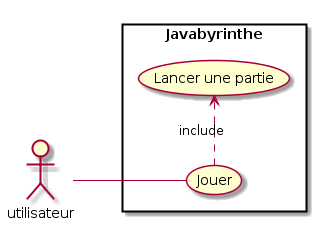
\includegraphics[width=15cm]{images/UML_casUtilisation_Javabyrinthe.png}%
	\caption{Diagramme de cas d'utilisation : Javabyrinthe}%
	\label{fig:useCase}%
\end{figure}
\newpage
\section{Jouer}
\begin{figure}[h!]%
\centering
	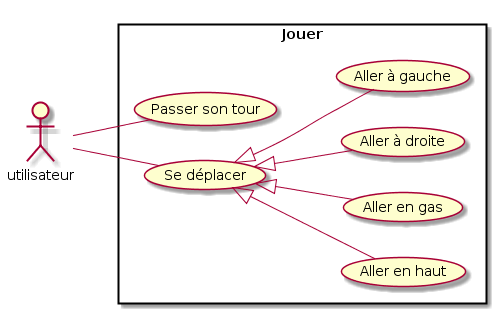
\includegraphics[width=15cm]{images/UML_casUtilisation_Jouer.png}%
	\caption{Diagramme de cas d'utilisation : Jouer}%
	\label{fig:useCase}%
\end{figure}

\section{LancementJeu}
\begin{figure}[h!]%
\centering
	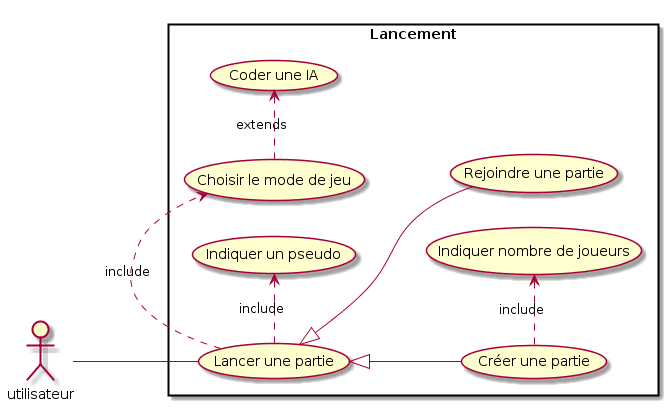
\includegraphics[width=15cm]{images/UML_casUtilisation_LancementJeu.png}%
	\caption{Diagramme de cas d'utilisation : Lancement Jeu}%
	\label{fig:useCase}%
\end{figure}


\chapter{Diagramme d'interactions}
	%\section{Diagramme de séquence}

\begin{figure}[h]%
	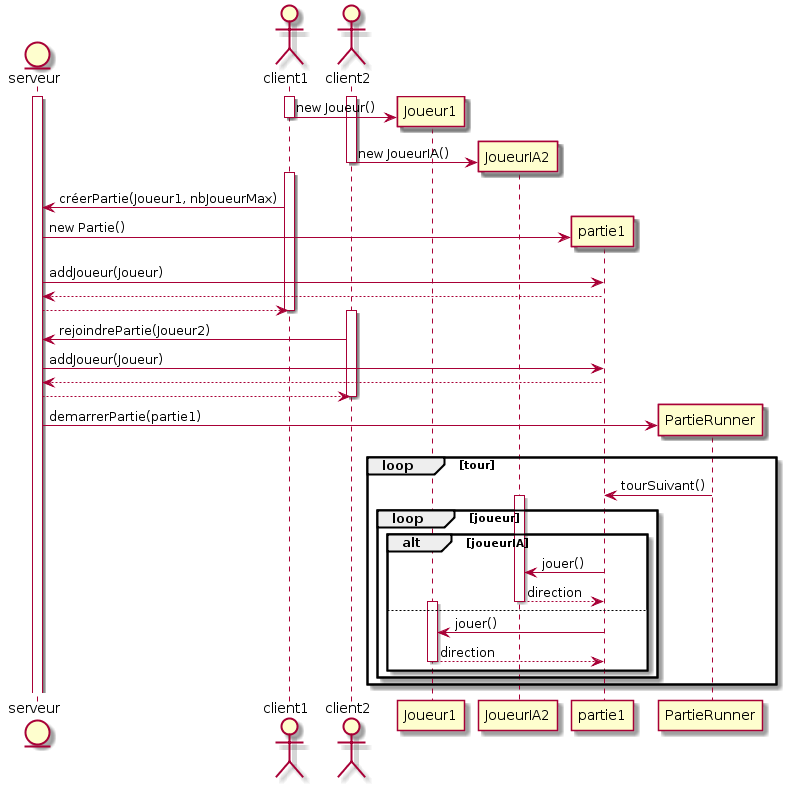
\includegraphics[width=\columnwidth]{images/UML_DiagSequence.png}%
	\caption{Diagramme de séquence}%
	\label{fig:useCase}%
\end{figure}

\chapter{Diagramme de classes}
	\begin{figure}[h]%
	\centering
	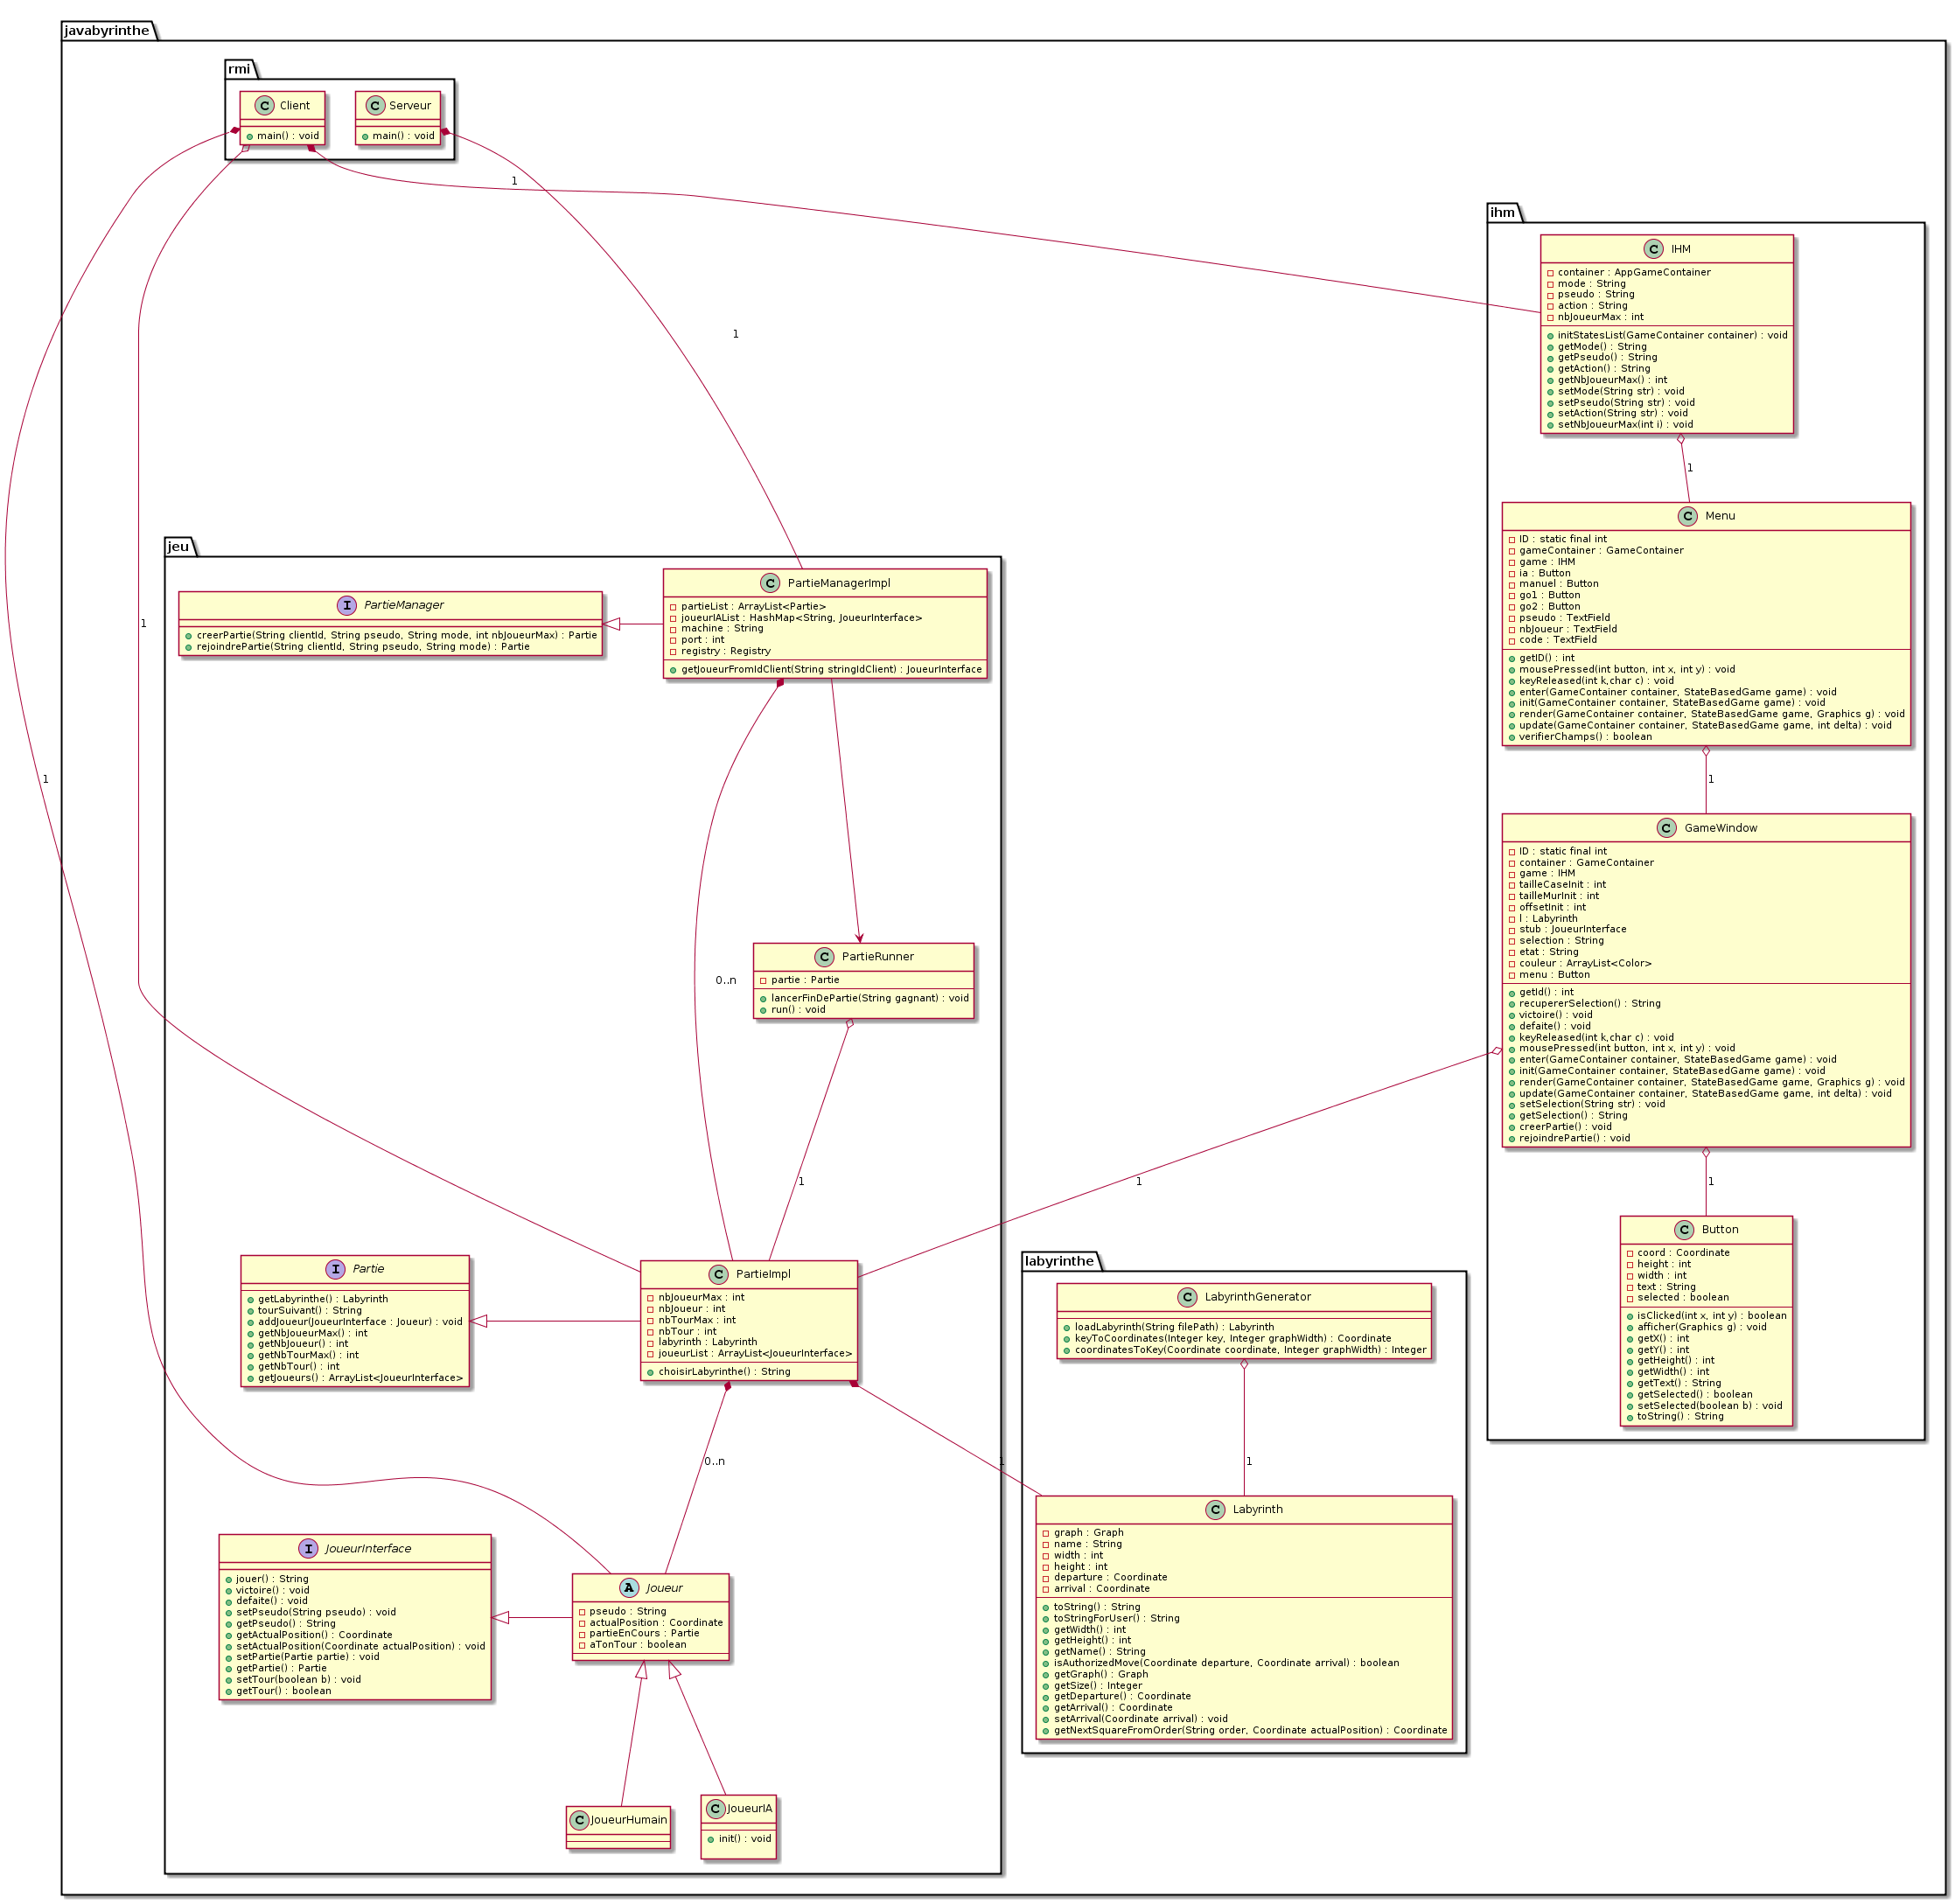
\includegraphics[height=18.5cm]{images/UML_diagClass.png}%
	\caption{Diagramme de classes}%
	\label{fig:diagClass}%
\end{figure}



\end{document}
